% ----- Consignes exo 1 ----- %
\begin{td-exo}[Points extrêmes]\,\\ % 1
	Soit \(P = \{x \in \bb R^2 : Ax\leq b, x\geq 0 \}\) avec 
    \begin{equation*}
        A = 
        \begin{pmatrix}
            1 & 1\\
            1 & -1
        \end{pmatrix}\quad \text{et}\quad
        b =
        \begin{pmatrix}
            3\\
            0
        \end{pmatrix}.
    \end{equation*}
    Combien y a-t-il de points extrêmes? Lister les points extrêmes et préciser si les points extrêmes sont des points dégénérés.
\end{td-exo}

% ----- Solutions exo 1 ----- %
\iftoggle{showsolutions}{
	\begin{td-sol}[]\ %
        Le polygone \(P\) est défini par les contraintes:
        \begin{equation*}
            \begin{alignedat}{2}
                \textcolor{red}{(1)}\quad & x_1 + x_2 &&\le 3 \\
                \textcolor{blue}{(2)}\quad & x_1 - x_2 &&\le 0 \\
                \textcolor{green!60!black}{(3)}\quad & x_1 &&\ge 0 \\
                \textcolor{orange}{(4)}\quad & x_2 &&\ge 0
            \end{alignedat}
        \end{equation*}
        Graphiquement, cela donne:
        
        \vspace{0.2cm}
        \ffigbox[\FBwidth]{%
\caption{\centering Représentation graphique des contraintes sur \(P\)}\label{Fig:cc_1_ex_1}
}{
    \fbox{
        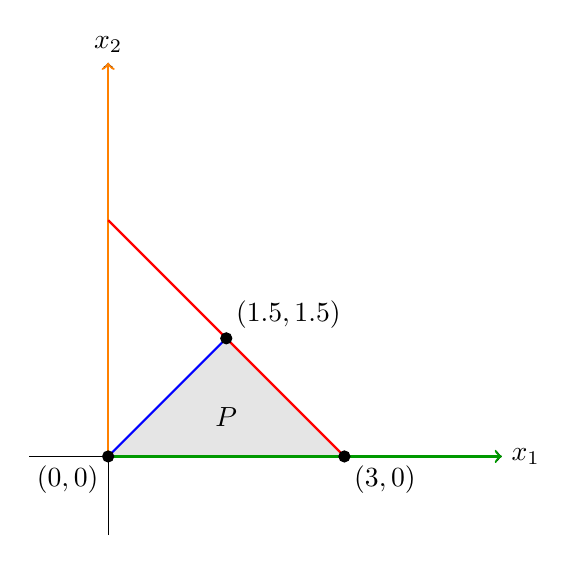
\begin{tikzpicture}[scale=1]
                % Feasible region
                \fill[black!10] (0,0) -- (1.5,1.5) -- (3,0) -- cycle;
                
                % Axes
                \draw[->] (-1,0) -- (5,0) node[right] {\(x_1\)};
                \draw[->, draw=green!60!black, thick] (0,0) -- (5,0) node[right] {};
                \draw[->] (0,-1) -- (0,5) node[above] {\(x_2\)};
                \draw[->, draw=orange, thick] (0,0) -- (0,5) node[above] {};
                
                
                % Constraints
                \draw[thick, draw=red] (0,3) -- (3,0) node[midway, above right] {};
                \draw[thick, draw=blue] (0,0) -- (1.5,1.5) node[midway, above left] {};
                
                
                % Points extrêmes 
                \filldraw[] (0,0) circle (2pt) node[below left] {\((0,0)\)};
                \filldraw[] (1.5,1.5) circle (2pt) node[above right] {\((1.5,1.5)\)};
                \filldraw[] (3,0) circle (2pt) node[below right] {\((3,0)\)};

                % Centre du polytope
                \node at (1.5,0.5) {\(P\)};
            \end{tikzpicture}
    }
}

        Les points extrêmes de \(P\) sont donc:
        \begin{itemize}
            \item \((0,0)\)
            \item \((1.5,1.5)\)
            \item \((3,0)\)
        \end{itemize}
        On voit alors clairement que 
        \begin{itemize}
            \item le point \((0,0)\) est dégénéré car trois contraintes sont actives en ce point, les contraintes \(\textcolor{blue}{(2)}\), \(\textcolor{green!60!black}{(3)}\) et \(\textcolor{orange}{(4)}\).
            \item le point \((1.5,1.5)\) n'est pas dégénéré car seules les contraintes \(\textcolor{red}{(1)}\) et \(\textcolor{blue}{(2)}\) sont actives en ce point.
            \item le point \((3,0)\) n'est pas dégénéré car seules les contraintes \(\textcolor{red}{(1)}\) et \(\textcolor{green!60!black}{(3)}\) sont actives en ce point.
        \end{itemize}
	\end{td-sol}
}{}


% ----- Consignes exo 2 ----- %
\begin{td-exo}[Ensembles et fonctions convexes]\, % 2
	\begin{enumerate}
        \item Soit \(S = \left\{ (x,y,z) \in \bb R^3 : z \geq x^2 + y^2 \right\}\). Montrer que \(S\) est un ensemble convexe.

        \item Soit \(C_1, C_2\) deux parties convexes d'un espace vectoriel réel \(E\) et soit \(s\in\ff{0,1}\).
        On pose \(C = sC_1 + (1-s)C_2 = \{ sx_1 + (1-s)x_2 : x_1 \in C_1, x_2 \in C_2 \}\).
        Montrer que \(C\) est convexe.

        \item Soit \(C_1\) et \(C_2\) deux ensembles convexes de \(\bb R^n\).
        On pose \(C = C_1 + C_2 = \{ x_1 + x_2 : x_1 \in C_1, x_2 \in C_2 \}\).
        Montrer que \(C\) est convexe.

        \item Soient \(f,g : \bb R \to \bb R\) deux fonctions convexes avec \(g\) croissante.
        Montrer que \(g \circ f\) est convexe.
    \end{enumerate}
\end{td-exo}

% ----- Solutions exo 2 ----- %
\iftoggle{showsolutions}{
    \begin{td-sol}[]\ %
        \begin{enumerate}
            \item Soient \((x_1,y_1,z_1), (x_2,y_2,z_2) \in S\) et \(\lambda \in [0,1]\).
            Montrons que le point \(\lambda (x_1,y_1,z_1) + (1-\lambda)(x_2,y_2,z_2)\) appartient à \(S\):
            \begin{equation*}
                \begin{aligned}
                    z &= \lambda z_1 + (1-\lambda) z_2 \\
                    &\geq \lambda (x_1^2 + y_1^2) + (1-\lambda)(x_2^2 + y_2^2) 
                    \quad \text{(car } z_1 \geq x_1^2+y_1^2 \text{ et } z_2 \geq x_2^2+y_2^2\text{)} \\ % chktex 9 chktex 1
                    &= \lambda x_1^2 + (1-\lambda)x_2^2 + \lambda y_1^2 + (1-\lambda)y_2^2 \\
                    &\geq {(\lambda x_1 + (1-\lambda)x_2)}^2 + {(\lambda y_1 + (1-\lambda)y_2)}^2 
                    \quad \text{(par l'inégalité (I))} \\
                    &= x^2 + y^2
                \end{aligned}
            \end{equation*}
            où \(x = \lambda x_1 + (1-\lambda)x_2\) et \(y = \lambda y_1 + (1-\lambda)y_2\). 

            On prouve en plus grand détail l'inégalité utilisée ci-dessus:
            
            \subsubsection*{Preuve de l'inégalité (I)}
            Pour tout \(\lambda \in [0,1]\) et tous réels \(a,b\), on a:
            \begin{equation*}
                \lambda a^2 + (1-\lambda) b^2 \geq {(\lambda a + (1-\lambda)b)}^2. \tag{I}
            \end{equation*}
            
            On a
            \begin{align*}
                &\lambda a^2 + (1-\lambda) b^2 - {(\lambda a + (1-\lambda)b)}^2 \\
                &= \lambda a^2 + (1-\lambda)b^2 - \left[ \lambda^2 a^2 + 2\lambda(1-\lambda)ab + {(1-\lambda)}^2 b^2 \right] \\
                &= \big(\lambda - \lambda^2\big) a^2 + \big((1-\lambda) - {(1-\lambda)}^2\big) b^2 - 2\lambda(1-\lambda)ab \\
                &= \lambda(1-\lambda) a^2 + \lambda(1-\lambda) b^2 - 2\lambda(1-\lambda)ab \\
                &= \lambda(1-\lambda) \left( a^2 + b^2 - 2ab \right) \\
                &= \lambda(1-\lambda) {(a-b)}^2 \geq 0.
            \end{align*}
            La dernière inégalité vient du fait que \(\lambda(1-\lambda) \geq 0\) pour \(\lambda \in [0,1]\), 
            et que \({(a-b)}^2 \geq 0\). 
            
            Ainsi, (I) est vérifiée. En l'appliquant à \(a=x_1, b=x_2\) puis à \(a=y_1, b=y_2\), 
            on obtient les inégalités nécessaires pour conclure que \(S\) est convexe.

            \item Soient \(x,y \in C\). Par définition de \(C\), il existe \(x_1,x_2 \in C_1\) et \(y_1,y_2 \in C_2\) tels que
            \begin{equation*}
                \begin{aligned}
                    x &= s x_1 + (1-s) x_2, \\
                    y &= s y_1 + (1-s) y_2.
                \end{aligned}
            \end{equation*}
            Soit \(\lambda \in [0,1]\). On a:
            \begin{equation*}
                \begin{aligned}
                    \lambda x + (1-\lambda) y 
                    &= \lambda \big( s x_1 + (1-s) x_2 \big) + (1-\lambda) \big( s y_1 + (1-s) y_2 \big) \\
                    &= \lambda s x_1 + \lambda (1-s) x_2 + (1-\lambda) s y_1 + (1-\lambda)(1-s) y_2 \\
                    &= s \big( \underbrace{\lambda x_1 + (1-\lambda) y_1}_{= x_0\in C_1} \big) + (1-s) \big( \underbrace{\lambda x_2 + (1-\lambda) y_2}_{= y_0\in C_2} \big)\\
                    &= s x_0 + (1-s) y_0 \in C.
                \end{aligned}
            \end{equation*}
            Ainsi, \(C\) est convexe.

            \item Soient \(x,y \in C\). Par définition de \(C\), il existe \(x_1,x_2 \in C_1\) et \(y_1,y_2 \in C_2\) tels que
            \begin{equation*}
                \begin{aligned}
                    x &= x_1 + x_2, \\
                    y &= y_1 + y_2.
                \end{aligned}
            \end{equation*}
            Soit \(\lambda \in [0,1]\). On a:
            \begin{equation*}
                \begin{aligned}
                    \lambda x + (1-\lambda) y 
                    &= \lambda (x_1 + x_2) + (1-\lambda)(y_1 + y_2) \\
                    &= \lambda x_1 + \lambda x_2 + (1-\lambda) y_1 + (1-\lambda) y_2 \\
                    &= \big( \underbrace{\lambda x_1 + (1-\lambda) y_1}_{= x_0\in C_1} \big) + \big( \underbrace{\lambda x_2 + (1-\lambda) y_2}_{= y_0\in C_2} \big)\\
                    &= x_0 + y_0 \in C.
                \end{aligned}
            \end{equation*}
            Ainsi, \(C\) est convexe.

            \item On rappelle que si \(f\) est convexe, alors pour tous \(x,y \in \bb R\) et \(\lambda \in [0,1]\), on a
            \begin{equation*}
                f \big( \lambda x + (1-\lambda) y \big) \leq \lambda f(x) + (1-\lambda) f(y).
            \end{equation*}
            Visuellement, la courbe de \(f\) est en dessous de la corde reliant les points \((x,f(x))\) et \((y,f(y))\).
            
            Soient \(x,y \in \bb R\) et \(\lambda \in [0,1]\).
            On a:
            \begin{equation*}
                \begin{aligned}
                    g \circ f \big( \lambda x + (1-\lambda) y \big) 
                    &= g \big( f(\lambda x + (1-\lambda) y) \big) \\
                    &\leq g \big( \lambda f(x) + (1-\lambda) f(y) \big) 
                    \quad \text{(car \(f\) est convexe)} \\
                    &\leq \lambda g(f(x)) + (1-\lambda) g(f(y)) 
                    \quad \text{(car \(g\) est convexe et croissante)} \\
                    &\leq \lambda (g \circ f)(x) + (1-\lambda)(g \circ f)(y).
                \end{aligned}
            \end{equation*}
            Ainsi, \(g \circ f\) est convexe.
        \end{enumerate}
    \end{td-sol}
}{}


% ----- Consignes exo 3 ----- %
\begin{td-exo}[Modélisation de contraintes]\, % 3
	Soient \(P_1,\ldots, P_n\) des propositions logiques, chécune étant vraie ou fausse.
    En introduisant des variables binaires, représenter les relations suivantes par des contraintes linéaires:
    \begin{enumerate}
        \item La proposition \(P_1\) est vraie.
        \item Toutes les propositions sont vraies.
        \item Au moins \(k\) propositions sont vraies.
        \item Si \(P_1\) est vraie, alors \(P_2\) est vraie.
        \item Les propositions \(P_1\) et \(P_2\) sont équivalentes.
        \item Si \(P_1\) ou \(P_2\) est vraie, alors au plus deux des propositions \(P_3,\ldots, P_n\) sont vraies.
    \end{enumerate}
    On pose \(x_i = 1\) si \(P_i\) est vraie, \(x_i = 0\) sinon.
\end{td-exo}

% ----- Solutions exo 3 ----- %
\iftoggle{showsolutions}{
	\begin{td-sol}[]\ %
        \begin{enumerate}
            \item \(x_1 = 1\).
            \item \(\sum_{i=1}^n x_i = n\).
            \item \(\sum_{i=1}^n x_i \geq k\).
            \item \(x_1 \leq x_2\) ou encore \(x_1 - x_2 \leq 0\).
            \item \(x_1 = x_2\) ou \(x_1 - x_2 = 0\).
            \item On peut utiliser une des deux formulations suivantes:
            \begin{itemize}
                \item On introduit une variable binaire \(y\) qui vaut 1 si \(P_1\) ou \(P_2\) est vraie, 0 sinon. On peut l'écrire comme suit:
                \begin{equation*}
                    y \geq x_1, \quad y \geq x_2, \quad y \leq x_1 + x_2.
                \end{equation*}
                La contrainte demandée s'écrit alors:
                \begin{equation*}
                    \sum_{i=3}^n x_i \leq 2 + (n-2)(1-y).
                \end{equation*}
                Si \(y=1\), alors la contrainte devient \(\sum_{i=3}^n x_i \leq 2\). Si \(y=0\), la contrainte devient \(\sum_{i=3}^n x_i \leq n\), qui est toujours vérifiée.

                \item On peut aussi écrire directement la contrainte:
                \begin{equation*}
                    \sum_{i=3}^n x_i \leq 2 + (n-2)(1 - x_1)(1 - x_2).
                \end{equation*}
                Si \(x_1=1\) ou \(x_2=1\), alors \((1 - x_1)(1 - x_2) = 0\) et la contrainte devient \(\sum_{i=3}^n x_i \leq 2\).
                Si \(x_1=0\) et \(x_2=0\), alors \((1 - x_1)(1 - x_2) = 1\) et la contrainte devient \(\sum_{i=3}^n x_i \leq n\), qui est toujours vérifiée.
            \end{itemize}
        \end{enumerate}
	\end{td-sol}
}{}


% ----- Consignes exo 4 ----- %
\begin{td-exo}[Résolution]\, % 4
	Soit le programme linéaire \(\mathcal{P}_0\) suivant:
    \begin{equation*}
        \mathcal{P}_0 = 
        \begin{cases}
            \max z(x) 35x_1 + 50x_2\\
            4x_1 + 6x_2 \leq 120\\
            x_1 + x_2 \leq 20\\
            2x_1 + 3x_2 \leq 40\\
            x_1, x_2 \geq 0
        \end{cases}
    \end{equation*}\,
    \begin{enumerate}
        \item Résoudre le problème \(\mathcal{P}_0\). 
        Donner les tableaux et les bases associées.

        \item Donner le dual de \(\mathcal{P}_0\).

        \item Donner la solution du dual à partir du tableau final du primal.

        \item Vérifier les écarts complémentaires.

        \item \texttt{Modification du vecteur} \(b\): le vecteur \(b\) devient \(b' = (75, 15, 50)\).

        \begin{enumerate}
            \item Que devient la solution optimale de \(\mathcal{P}_0\)?

            \item Proposer deux méthodes pour résoudre ce nouveau problème,
            sans tenter de résoudre le dit problème.
        \end{enumerate}
    \end{enumerate}
\end{td-exo}

% ----- Solutions exo 4 ----- %
\iftoggle{showsolutions}{
	\begin{td-sol}[]\ %
		
	\end{td-sol}
}{}


% ----- Consignes exo 5 ----- %
\begin{td-exo}[Farkas]\, % 5
	Est-ce que les systèmes suivants admettent une solution?
    \begin{enumerate}
        \item On résoud \(Ax \leq b, x \geq 0\) avec
        \begin{equation*}
            A =
            \begin{pmatrix}
                1 & 1\\
                -1 & 0\\
                0 & -1
            \end{pmatrix}\quad \text{et}\quad
            b =
            \begin{pmatrix}
                1\\
                0\\
                0
            \end{pmatrix}.
        \end{equation*}

        \item On résoud \(Ax \leq b, x \geq 0\) avec
        \begin{equation*}
            A =
            \begin{pmatrix}
                1 & 1 & 1\\
                1 & 0 & 0\\
                0 & 3 & 1\\
                0 & 0 & 1
            \end{pmatrix}\quad \text{et}\quad
            b =
            \begin{pmatrix}
                8\\
                4\\
                12\\
                6
            \end{pmatrix}.
        \end{equation*}

        \item On résoud \(Ax = b, x \geq 0\) avec
        \begin{equation*}
            A =
            \begin{pmatrix}
                -2 & 3 & 0\\
                1 & -1 & 2
            \end{pmatrix}\quad \text{et}\quad
            b =
            \begin{pmatrix}
                1\\
                -1
            \end{pmatrix}.
        \end{equation*}
    \end{enumerate}
\end{td-exo}

% ----- Solutions exo 5 ----- %
\iftoggle{showsolutions}{
	\begin{td-sol}[]\ %
		
	\end{td-sol}
}{}

